\documentclass[aps, pre, onecolumn, nofootinbib, notitlepage, groupedaddress, amsfonts, amssymb, amsmath, longbibliography, superscriptaddress]{revtex4-1}
\usepackage{tabularx}
\usepackage{graphicx}
\usepackage{hyperref}
\usepackage{xcolor}
\hypersetup{
    colorlinks,
    linkcolor={red!50!black},
    citecolor={blue!50!black},
    urlcolor={blue!80!black}
}
\usepackage{bm}
\usepackage{natbib}
\usepackage{longtable}
\LTcapwidth=0.87\textwidth

\newcommand{\Div}[1]{\ensuremath{\nabla\cdot\left( #1\right)}}
\newcommand{\DivU}{\ensuremath{\nabla\cdot\bm{u}}}
\newcommand{\angles}[1]{\ensuremath{\left\langle #1 \right\rangle}}
\newcommand{\KS}[1]{\ensuremath{D_{\text{KS}}(#1)}}
\newcommand{\KSstat}[1]{\ensuremath{\overline{D_\text{KS}(#1)}}}
\newcommand{\grad}{\ensuremath{\nabla}}
\newcommand{\RB}{Rayleigh-B\'{e}nard }
\newcommand{\Reff}{\ensuremath{\text{Re}_{\text{ff}}}}
\newcommand{\Peff}{\ensuremath{\text{Pe}_{\text{ff}}}}
\newcommand{\stressT}{\ensuremath{\bm{\bar{\bar{\Pi}}}}}
\newcommand{\lilstressT}{\ensuremath{\bm{\bar{\bar{\sigma}}}}}


\newcommand\mnras{{MNRAS}}%
\newcommand\apjl{{The Astrophysical Journal Letters}}%

\begin{document}
%\author{Evan H. Anders}
%\affiliation{Dept. Astrophysical \& Planetary Sciences, University of Colorado -- Boulder, Boulder, CO 80309, USA}
%\affiliation{Laboratory for Atmospheric and Space Physics, Boulder, CO 80303, USA}

\title{Additions to ch3 postscript}

\maketitle

%%%%%%%%%%%%
%%%%%%%%%%%
% INTRO
%%%%%%%%%%%
%%%%%%%%%%%%

\section{Concerns}
These concerns are copied and pasted from Brad's email on march 23:
\begin{enumerate}
\item How do you calculate your Rossby number?  Is it a volumetric average?  Temporal average? Are you averaging the enstrophy and taking the square root? Are you averaging the modulus of the vorticity?
\item So, your epsilon is rather tiny. You informed me previously that the models barely restratify for small epsilon.  Is that true when the model is rotationally constrained?
\item How big of an unstable band of wavenumber do you expect to see?  Your boxes seem a little narrow to me.  Your horizontal spectral resolution is pretty poor in the sense that you should only get three discrete nonzero wavenumbers that are smaller than the critical onset wavenumber.  I can't decide if this is a problem or not.
\item The equation at the end of page 56 has got something wrong. Are you saying that Keith's expression (Nu-1) $\sim$ Ra$^{3/2}$ Ta$^{-1}$ is equivalent to Ra / Ra$_\text{crit}^{1/6}$ ?  That is clearly not right since Ta $\sim$ Ra$_{\text{crit}}^{3/2}$ . I have lost your argument somewhere in the middle of this equation.
\item So, you mention repeated the scaling achieved by King et al. (2012), which has a theoretical argument for why it exists.  Are your models consistent with the assumptions that King et al. use? i.e., Do your boundary layers scale like $\delta_s \sim \text{Ra}^{-1/3}$?
\item You also discuss the Ra$\sim$Ta$^{3/4}$ scaling of Julien et al. 2012. I am completely confused.  Both of the Rayleigh and Taylor numbers are inputs.  They can't scale.
\item You might want to derive the scaling law that figure 3.5 suggests. My quick estimate gives Ro ~ Ek$^{1/3}$.  That doesn't seem "weak" to me since lots of dynamics scale with similar power laws.  For example, the most unstable wavenumber scales like Ek$^{-1/3}$.
\end{enumerate}

\section{Quick Responses}

\begin{enumerate}
\item We calculate:
$$
\text{Ro} = \frac{\sqrt{\bm{\omega}\cdot\bm{\omega}}}{2 \Omega},
\qquad\text{with}\qquad
\bm{\omega} = \grad\times\bm{u}.
$$
everywhere in the domain.
We then take a volume average
$$
\angles{\text{Ro}} = \frac{1}{L_x L_y L_z}\iiint \text{Ro}\,dx\,dy\,dz,
$$
and output that quantity to file.
To get the values reported in the paper, we take a time-average of the volume average,
$$
\text{Ro}_{\text{reported}} = \frac{1}{t_2 - t_1}\int_{t_1}^{t_2} \angles{\text{Ro}} dt.
$$
\item Even in rotationally constrained systems, the initial stratification is the same as evolved stratification to within $\sim\epsilon$ (see Fig.~\ref{fig:rot_density}). 
So the flows do feel $\sim$3 density scale heights in this work. 
\begin{figure}[t!]
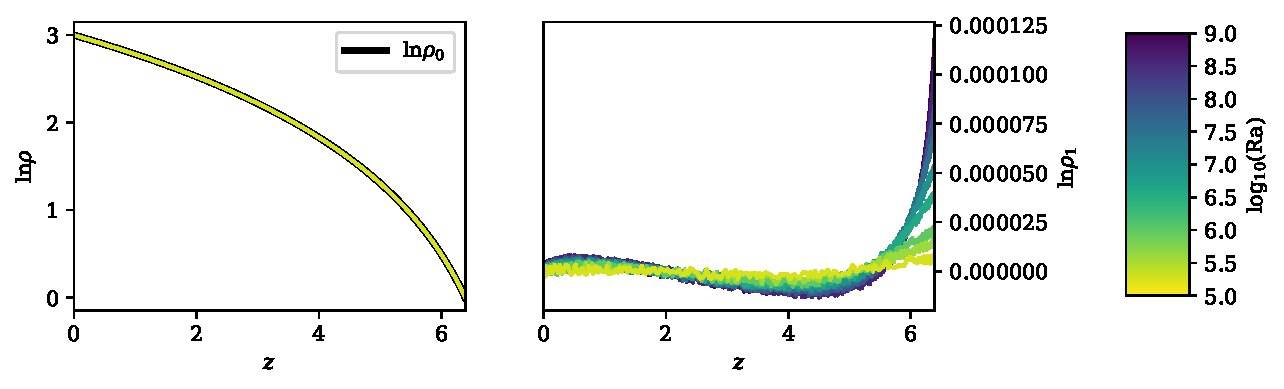
\includegraphics[width=\textwidth]{./figs/rot_density.pdf}
\caption{ 
	Density profiles for all simulations with Ro$_{\text{p}} = 0.6$ are shown.
	(Left) The log of the full density profile compared to the initial profile.
	All profiles are, to first order, indistinguishable from the initial profile.
	(Right) Deviations in $\ln\rho$ away from the initial state.
	As Ra increases (from yellow to purple), density differences, particularly in the upper boundary layer, become more extreme.
	The noise in these profiles is a result of the accuracy of the output data that I have on hand (which was the full rho profile, not the fluctuations), and does not reflect noise or accuracy in the simulations themselves.
	\label{fig:rot_density} }
\end{figure}

\item See Fig.~\ref{fig:ta1e10_onset}. 
Intuitively, I agree -- our boxes seem a little narrow, however, the most unstable and fastest-growing horizontal modes are certainly contained within our simulation domain.
Visually, flows in our simulations do not appear to be dominated by low-aspect-ratio effects (e.g., development of mean flows driven by convective elements not having enough room to horizontally expand).
From a private conversation with Jon Aurnou (2019 APS Division of Fluid Dynamics meeting), I expressed a similar concern: perhaps our simulation boxes were too narrow, and that led to confusing results.
He has quite a bit more experience and intuition for rotating convection than I do, and he didn't seem concerned by our choice.
His intuition is essentially that rotationally constrained convective domains become ``infinitely large'' compared to convective elements very quickly.
Due to rotationally constrained structures becoming essentially vertically invariant, the difference between a large box and a small box is whether you fit a lot or a few of those vertically invariant structures into your box.
But -- the solution and heat transport per horizontal area should be the same.
It's unclear if that intuition fits in stratified convection, but our highly-rotationally constrained results (right panels of Fig.~3.2) suggest that even stratified domains can achieve mostly vertically invariant flows.
\begin{figure}[t!]
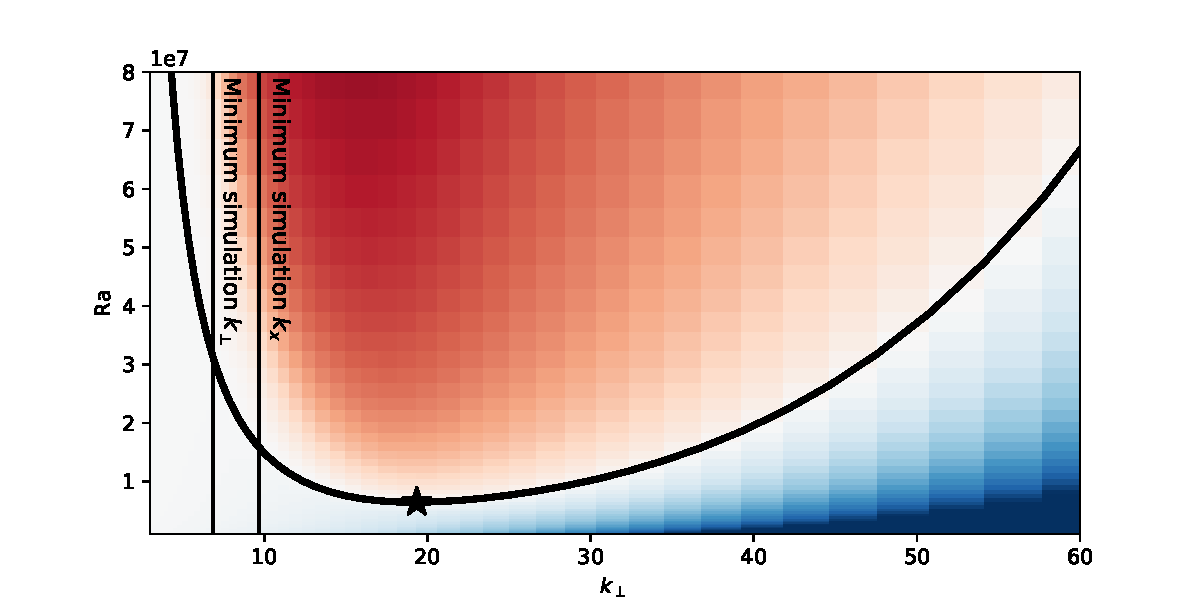
\includegraphics[width=\textwidth]{./figs/crit_curve_ta1e10.pdf}
\caption{ 
	Critical curve of convective onset at Ta = $10^{10}$, $\epsilon = 10^{-4}$, $n_\rho = 3$.
	Red colors indicate a value of $(k_\perp, \text{Ra})$ that is convectively unstable -- that is, where the linear solution is exponential growth.
	Blue colors indicate a linear solution of exponential decay.
	The thick black line shows the critical curve that separates convectively unstable modes from convectively stable modes.
	The star indicates the true value of the critical Rayleigh number and indicates the point $(k_{\perp, \text{crit}}, \text{Ra}_{\text{crit}})$.
	In our simulation domains, we set $L_x = L_y = 2 \lambda_\text{crit} = 4\pi / k_{\perp, \text{crit}}$.
	For this choice, we have annotated the maximum wavenumber which is contained along a given horizontal direction ($x$ or $y$) with a line (``Minimum simulation $k_x$''), as well as the maximum wavenumber contained along a diagonal of our simulation (``Minimum simulation $k_\perp$'').
	\label{fig:ta1e10_onset} }
\end{figure}
\item Ah, the confusion here is due to bad notation on our part.
The Ra$_{\text{crit}}$ we're referring to here is a Ra$_{\text{crit}}(\text{Ro}_{\text{p}})$, not a Ra$_{\text{crit}}(\text{Ta})$.
If you look at Fig.~ 3.1a, we're referring to the value of Ra$_{\text{crit}}$ for a given value of $\text{Ro}_\text{p}$, which has a singular value, indicated by an orange circle.
We're not referring to the full black line in that figure which is Ra$_{\text{crit}}(\text{Ta})$.
Perhaps we should have stopped that scaling before the final proportionality and left it at (Nu − 1) $\propto \text{Ra}^{3/2} / \text{Ta} = \text{Ro}_{\text{p}} \text{Ra}^{1/6}$, meaning that we would expect a Ra$^{1/6}$ scaling along a fixed Ro$_{\text{p}}$ path.
\item To first order, $\delta_s \sim \text{Ra}^{-1/3}$ is a good description of what we're seeing on our Ro$_\text{p}$ paths.
See Fig.~\ref{fig:ro_p_boundary_layers}.
\begin{figure}[t!]
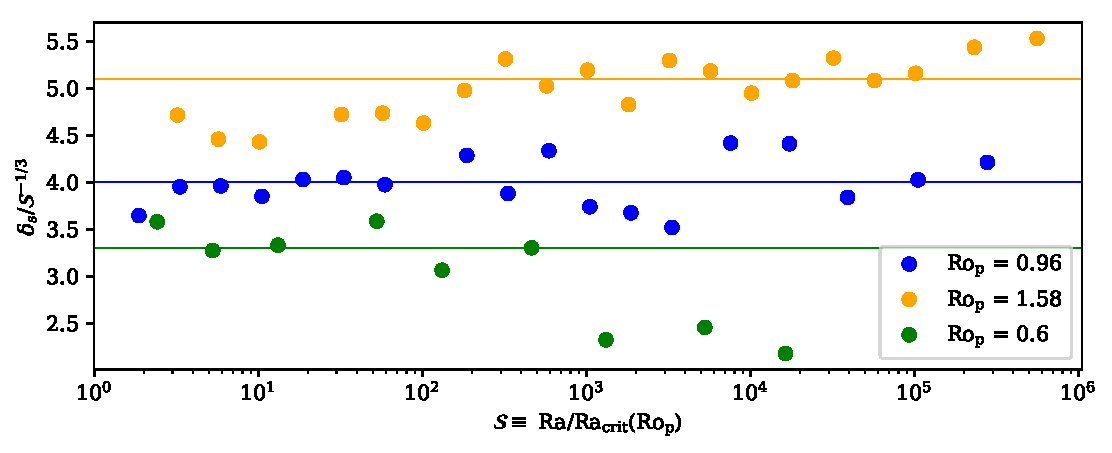
\includegraphics[width=\textwidth]{./figs/ro_p_boundary_layers.pdf}
\caption{ 
	The thickness of the entropy boundary layer at the top of the simulation is plotted vs.~Ra at constant Ro$_{\text{p}}$.
	For each case, we plot the supercriticality, $\mathcal{S}$ on the x-axis, which is Ra normalized by the value of Ra$_{\text{crit}}$ along that Ro$_{\text{p}}$ path, reported in table 3.1.
	The boundary layer values are compensated by $\mathcal{S}^{-1/3}$, the prediction for the scaling of boundary layers per the arguments of King et.~al.
	To first order, across many decades of Ra, this quantity is flat, indicating that this predition describes our simulation behavior well.
	\label{fig:ro_p_boundary_layers} }
\end{figure}
\item At fixed Prandtl number (and $\epsilon$, $n_\rho$), the solution is completely characterized by Ra and Ta -- correct.
We've posited in this work that there's a ``new'' input parameter,
\begin{equation}
\text{Ro}_\text{p} = \text{Ra}^\alpha\text{Ta}^\beta\text{Pr}^{\gamma}.
\end{equation}
Rearranging this expression, it becomes clear that
\begin{equation}
\text{Ta} = \left(\text{Ra}^\alpha\text{Pr}^{\gamma}\right)^{1/\beta},
\end{equation}
which is to say that, at fixed Pr, even if we now have ``three'' input parameters (Ra, Ta, Ro$_{\text{p}}$), we only have two degrees of freedom given those inputs.
Choosing two (e.g., Ra and Ro$_\text{p}$ in this work) specifies the third (Ta).

We've suggested that $\alpha = 1/2$, $\beta = -3/8$, and $\gamma = -1/4$ may be the ``proper'' definition of Ro$_{\text{p}}$, where by ``proper'' we mean: these exponents may trace out surfaces in (Ra, Ta, Pr) space along which the Rossby number is constant.
When we refer to the Ra$\sim$Ta$^{3/4}$ scaling, what we are referring to is really the ratio of $\beta$ and $\alpha$,
$$
\frac{\beta}{\alpha} = \frac{-3/8}{1/2} = -\frac{3}{4}.
$$
Recast differently, if you fix the values of Pr and Ro$_{\text{p}}$, you can see that Ra and Ta are constrained by
$$
\text{Ra} \propto \text{Ta}^{-\beta/\alpha} \qquad\rightarrow\qquad
\text{Ra} \propto \text{Ta}^{3/4},
$$
and this is the scaling we're referring to.
\item This work is hugely preliminary, but Ben Brown (private communication, Mar.~25, 2020) was able to get me the exact values that went into making this figure.
They are presented in Table~\ref{table:rop_spheres}.
These simulations reportedly take a very long time to converge, and these results are extremely preliminary (benchmarking, etc.~ is underway to ensure that they are trustworthy).
Ben claims that it's probably not reasonable to have faith in the runs that haven't evolved for more than 5 viscous diffusion timescales (at the top of the domain), so I'm dropping those points from further analysis.
It's unclear if the points that have run for fewer than 20 viscous timescales are trustworthy in his opinion, but for now I'm going to assume that they are.
I've re-plotted the `trustworthy' points in the left panel of Fig.~\ref{fig:mdwarfs_rop}.
The points with Ro$_\text{p}^2 > 20$ seem to have a sensible scaling, and the best fit law is roughly $\text{Ro} \sim \text{Ro}_\text{p}^2 \text{Ek}^\alpha$ where $\alpha \approx 0.25$ for Ro$_\text{p}^2 = 80$ and $\alpha \approx 0.22$ for Ro$_\text{p}^2 = \{20, 40\}$.
In the right panel of Fig.~\ref{fig:mdwarfs_rop}, I've compensated this plot by an Ek$^{0.22}$ scaling law, and I've normalized all points by their value at Ek$ = 3 \times 10^{-3}$ to show the goodness of these power-law fits.
Indeed, in these data, even at fixed Ro$_\text{p}$, the evolved Rossby number has a fairly large ($\alpha \sim 1/4$) Ek dependence remaining.
It's unclear to me if this is due to geometry effects, or if it is due to the region of parameter space that these models are in.
We previously found that Ro$_\text{p}$ behaved best for low Ro cases (at lower Ek than these runs), and the lowest Ro points here behave very strangely.
Further data is needed to determine if Ro$_{\text{p}}$ works well in spherical domains.




\begin{figure}[ht!]
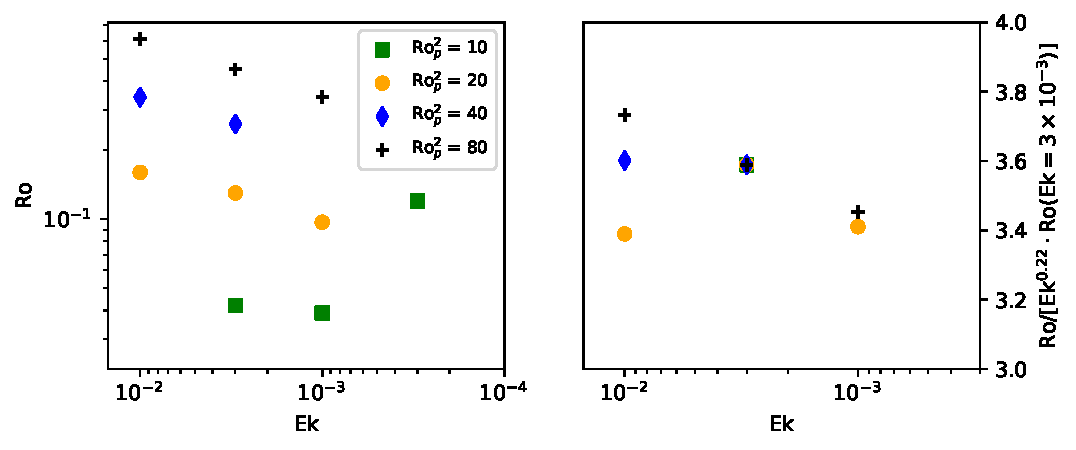
\includegraphics[width=\textwidth]{./figs/mdwarfs_rop.pdf}
\caption{ (left) Ro vs.~Ek from preliminary dynamo models in spherical domains which include the $r = 0$ point.
		  (right) A compensated Ro vs.~Ek plot, where an Ek$^{0.22}$ law has been removed from the data, and where the data has been normalized by the value of Ro at Ek = $3 \times 10^{-3}$.
	\label{fig:mdwarfs_rop} }
\vspace{-0.75cm}
\end{figure}



\begin{table}[htb]
    \caption[Preliminary Rossby numbers in Mdwarf simulations.]{
	Results from preliminary dynamo models are reported.
	The squared value of Ro$_\text{p}$ and the value of Ek (input values) are reported, as well as the evolved value of Ro and the total simulation run time in units of viscous diffusion timescales at the top of the domain.
	Due to diffusivities decreasing with depth (and increasing density), the viscous diffusion timescale is much longer at the bottom of the domain (at $r = 0$).
	}
    \begin{center}
    \begin{tabular}{c c c c} \hline
	Ro$_\text{p}^2$ & Ek &  Ro & run time ($t_{\text{visc, top}}$) \\
	\hline
	10	&	$3 \times 10^{-3}$	& 0.042 & 	20	\\
	10	&	$10^{-3}$			& 0.039	&	9.6 \\
	10 	&	$3 \times 10^{-4}$	& 0.12	&	6.8 \\
	20	&	$10^{-2}$			& 0.16	&	20 \\
	20	&	$3 \times 10^{-3}$	& 0.13	&	20 \\
	20	&	$10^{-3}$			& 0.097 &	20 \\
	20 	&	$8 \times 10^{-4}$	& 0.088	&	4.6 \\
	20	&	$5 \times 10^{-4}$	& 0.079 &	2.3 \\
	40	&	$10^{-2}$			& 0.34	&	20  \\
	40	&	$3 \times 10^{-3}$	& 0.26	&	20  \\
	40	&	$10^{-3}$			& 0.19	&	3.3 \\
	80	&	$10^{-2}$			& 0.61	&	20  \\
	80	&	$3 \times 10^{-3}$	& 0.45	&	20  \\
	80	&	$10^{-3}$			& 0.34	&	10	\\
	80	&	$3 \times 10^{-4}$	& 0.26	&	0.41 \\
	\end{tabular}
\end{center}
\label{table:rop_spheres}
\end{table}



\end{enumerate}

\end{document}
